\documentclass[11pt]{article}

\usepackage[margin=1in]{geometry}
\usepackage{amsmath,amssymb}
\usepackage{xcolor}
\usepackage[hidelinks]{hyperref}
\usepackage{enumitem}
\usepackage{graphicx}
\usepackage{tikz}
\usepackage{tikz}

\title{2024 F=ma Exam Review}
\author{Nathan P.}
\date{February 4, 2026}

\begin{document}
\maketitle

\subsection*{Question 2}
\begin{itemize}[leftmargin=*]
\item The walls are frictionless, and usually with the vertical walls it’s the friction that keeps you from falling downward, while in this case it’s the vertical component of normal force.
\end{itemize}

\subsection*{Question 3}
\noindent
\begin{minipage}[t]{0.72\linewidth}
  \begin{itemize}[leftmargin=*]
  \item Balance horizontal and vertical forces at each point, starting at C bc we know a force is applied there.
  \item Draw it out; don’t just rely on your brain to keep track of everything.
  \end{itemize}
\end{minipage}\hfill
\begin{minipage}[t]{0.4\linewidth}
  \vspace{2pt}
  \vspace{-3\baselineskip}
  \includegraphics[width=0.7\linewidth]{q3.png}
\end{minipage}

\subsection*{Question 7}
\begin{itemize}[leftmargin=*]
\item $v=at$, $x=\tfrac12 at^2$, so plugging in $t$ in terms of $x$ into $v=at$ gives $v \propto \sqrt{x}$.
\item Another way: $dv/dt = k$ (constant as we can see from $v$-$t$ graph), $k = dv/dx \, v$, $dv/dx=k/v$, so slope of $dv/dx$ decreases as $v$ increases and vice versa.
\end{itemize}

\subsection*{Question 8}
\begin{itemize}[leftmargin=*]
\item The midpoint of a rod sliding down a frictionless wall has the average of the velocities of the endpoints, i.e. $0.5(\vec{v}_{\text{top}} + \vec{v}_{\text{bot}})$.
\item For the $45^\circ$ case it’s $((v,0)+(0,-v))/2=(v/2,-v/2)$ which has magnitude $v\sqrt{(1/2)^2+(1/2)^2}=v/\sqrt{2}$, a.k.a. a $45$-$45$-$90$ triangle.
\end{itemize}

\subsection*{Question 11}
\begin{itemize}[leftmargin=*]
\item Force = Difference in the pressure from outside and inside $\times$ \text{Surface area of one hemisphere:} $F=\Delta PA$.
\end{itemize}

\subsection*{Question 13}
\begin{itemize}[leftmargin=*]
\item $T$ as a function of $x$, not $T$ over time.
\item Key: use limiting cases. If $x=0$ then $T=mg$ bc they’re equal masses. If $x\to\infty$ then it’s like a table pulley, $T$ is horizontal for left block and $T=mg/2$, so B is the graph that matches.
\end{itemize}

\subsection*{Question 14\textsuperscript{\textcolor{blue}{\href{https://math-gpt.org/video/hls_00eb09bd-45c9-4a77-aef1-9a6ecba4cbe7}{1}}}}
\begin{itemize}[leftmargin=*]
\item “Stop moving wrt” the hoop means they move at the same velocity. Conserving horizontal momentum, that velocity must be half the initial.
\item Conserve energy: start with only bead $m$ moving, then the whole $2m$ moving at $v/2$ + some $mgh$ of the bead. Solve for $h$.
\item Find what angle that corresponds to: geometry shows $h=R(1-\cos\theta)$.
\end{itemize}

\subsection*{Question 16}
\begin{itemize}[leftmargin=*]
\item Initial speed when released also depends on $g$; it’s not the same for both on earth and on moon. I also didn’t realize $d$ shouldn’t depend on $g$ ($\text{m}/\text{s}^2$) based on dimensions of given variables that $d$ must be a function of.
\item If the point of release is at height $h$, $v^2=2gh$ there (energy) and $d \propto v^2/g$ so $g$ cancels out.
\end{itemize}

\subsection*{Question 17}
\begin{itemize}[leftmargin=*]
\item One thing at a time. Balance force on bottom string/spring, then consider pulley movement, then balance forces on top string/springs.
\item Use conservation of string and consider spring stretches to find relation for total displacement of the mass.
\end{itemize}

\subsection*{Question 18}
\begin{itemize}[leftmargin=*]
\item Set up energy conservation right after finish firing, so you have new speed + potential at that point = total energy.
\item No need to consider at apogee, bc we’re asked for $\Delta v$ so we need $v_f$ and $v_i$ which can be found at same point perigee, and that point is $R$ away from planet which is convenient.
\end{itemize}

\subsection*{Question 19}
\begin{itemize}[leftmargin=*]
\item My mistakes: treating the rods as point masses at their com for calculating $I$. I cannot do that. They are $1/3\,mr^2$ from the end. Another mistake was forgetting to use total mass $7m$ for $\omega=\sqrt{mdg/I}$.
\item Redoing the problem with those fixes yields the correct answer.
\item It’s a physical pendulum, so just find $I$ and $d$ (distance from pivot to cm) and plug into $\omega=\sqrt{mgd/I}$.
\end{itemize}

\subsection*{Question 20}
\begin{itemize}[leftmargin=*]
\item Key idea: if vertical masses move by $x$, horizontal masses must move by $x$. Just consider one rod; conserving rod length is just like the case where a rod slides down a wall.
\item Then think energy! Bc we have forces in diff directions, but energy still involves $m$ and $k$ and don’t deal with directions so we’re going with that! Write out expression for total energy $K+U$ and notice the pattern—effectively one spring-mass system with mass $4m$ and spring constant $8k$ (2 $k$’s compressed 2x).
\end{itemize}

\subsection*{Question 21}
\begin{center}
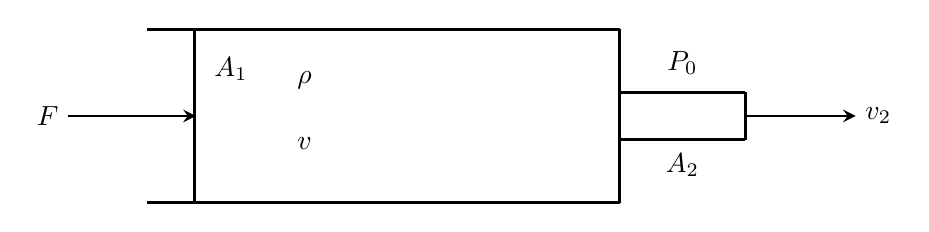
\begin{tikzpicture}[x=1cm,y=1cm,>=stealth]
  % duct outline
  \draw[line width=1.2pt] (0,0) -- (6,0);
  \draw[line width=1.2pt] (0,2.2) -- (6,2.2);
  % right contraction / nozzle
  \draw[line width=1.2pt] (6,0) -- (6,2.2);
  \draw[line width=1.2pt] (6,0.8) -- (7.6,0.8);
  \draw[line width=1.2pt] (6,1.4) -- (7.6,1.4);
  \draw[line width=1.2pt] (7.6,0.8) -- (7.6,1.4);

  % left section marker (A1)
  \draw[line width=1pt] (0.6,0) -- (0.6,2.2);
  \node[anchor=east] at (1.4,1.7) {$A_1$};

  % flow properties inside
  \node at (2.0,1.55) {$\rho$};
  \node at (2.0,0.75) {$v$};

  % force arrow on left
  \draw[->,line width=1pt] (-1.0,1.1) -- (0.62,1.1);
  \node[anchor=east] at (-1.0,1.1) {$F$};

  % P0, A2, v2
  \node[anchor=south] at (6.8,1.5) {$P_0$};
  \node[anchor=north] at (6.8,0.75) {$A_2$};
  \draw[->,line width=1pt] (7.6,1.1) -- (9.0,1.1);
  \node[anchor=west] at (9.0,1.1) {$v_2$};
\end{tikzpicture}
\end{center}
\begin{itemize}[leftmargin=*]
\item Set up Bernoulli’s; $v_2$ is unknown so use continuity equation to express it in terms of the givens, plug it in, solve for $F$.
\item Use approximation (problem explicitly mentions approximate) $A_1\gg A_2$ so the $-1$ drops out in $(A_1^2/A_2^2 -1)$.
\end{itemize}

\subsection*{Question 23}
\begin{itemize}[leftmargin=*]
\item Find coefficient of restitution $e=v'/v$ which happens to be $1/\sqrt{2}$ since half energy is lost so $v$ decreases by factor of $\sqrt{2}$.
\item Key: must come in and go out at speed $v$ to be “bouncing steadily” and reach the same new height.
\item Then apply that same $e$ in the paddle frame, where $v_{\text{in}} = v+1$ and $v_{\text{out}}=v-1$, solve for $v$.
\item $h=v^2/2g$.
\end{itemize}

\subsection*{Question 24}
``when reached half of its terminal velocity'' implies $F_g \approx F_d$, so find what each is proportional to and set equal

since $F_{\text{drag}} \propto v^2$ and $v^2=2gd$ for small $d$, plug that into $F_{\text{drag}}$

\subsection*{Question 25}
decreases in magnitude, then increases in magnitude when acceleration flips to be upward

$\omega=v/r$, as $r$ decreases $\omega$ increases and $K_r$ takes up more of the energy from dropping down

\begin{itemize}[leftmargin=*]
\item ``When reached half of its terminal velocity'' implies $F_g \approx F_d$, so find what each is proportional to and set equal.
\item Since $F_{\text{drag}} \propto v^2$ and $v^2=2gd$ for small $d$, plug that into $F_{\text{drag}}$.
\end{itemize}

\subsection*{Question 25}
\begin{itemize}[leftmargin=*]
\item Decreases in magnitude, then increases in magnitude when acceleration flips to be upward.
\item $\omega=v/r$, as $r$ decreases $\omega$ increases and $K_r$ takes up more of the energy from dropping down.
\item Basically, a dropping yoyo speeds up then slows down translationally.
\end{itemize}

\end{document}
